%%%%%%%%%%%%%%%%%%%%%%%%%%%%%%%%%%%%%%%%%%%%%%%%%%%%%%%
%
% sample root file for a contribution.
% you can adjust this sample file for convenience.
%
%%%%%%%%%%%%%%%%%%%%%%%%%%%%%%%%%%%%%%%%%%%%%%%%%%%%%%%

%
% >>>>>>>>>>>>>>> PLEASE NOTE <<<<<<<<<<<<<<<
%
% This file is not stand-alone compileable as it is, to make it compileable during development uncomment the preamble below.
% In this case, you also have to uncomment the begin/end document statements.
% Don't forget to comment it the preamble and the begin/end document statements again or erase them when handing in your contribution.
%
% If you use BibTex for your bibliography, please use \putbib[bibliography] to print your reference (see end of this file).
%
% you can use paths relative to your chapter dir in most commands like \input, \figure, etc., e.g. \figure{assets/fig1}.
%
% as this is a contribution, please prefix references with a unique sequence to avoid clashes between chapters, for instance with your chapter number or your name, e.g. \label{01:myheading} or \label{mueller:myheading}.
%
% >>>>>>>>>>>>>>>>>>>><<<<<<<<<<<<<<<<<<<<<<<

%%%%%%%%%%%%%%%%%%%%%%%%%%%%%%%%%%%%%%%%%%%%%%%%%%
%% you can uncomment the following preamble during development to make this file compileable.
%% Note that you need the svmult.cs file inside your chapter root dir to make this work.
%% Also note that if you need additional packages etc., you can add them here, but 
%% please notify the editor of the book so it'll be added to the book in the end.
%% When you hand in your contribution, please uncomment or remove the preamble again.
%%%%%%%%%%%%%%%%%%%%%%%%%%%%%%%%%%%%%%%%%%%%%%%%%%
%%%%%%%%%%%%%%%%%%%%%%%%%%%%%%%%%%%%%%%%%%%%%%%%%%%
%\documentclass[
%graybox,
%envcountchap,
%%natbib
%]{svmult}
%
%%\usepackage{type1cm}        % activate if the above 3 fonts are 
%% not available on your system
%
%\usepackage{makeidx}         % allows index generation
%\usepackage{graphicx}        % standard LaTeX graphics tool
%% when including figure files
%\usepackage{multicol}        % used for the two-column index
%\usepackage[bottom]{footmisc}% places footnotes at page bottom
%
%\usepackage{newtxtext}       % 
%\usepackage{newtxmath}       % selects Times Roman as basic font
%
%% \usepackage{ natbib}
%\usepackage{footmisc}
%
%%% Additional packages added. Add necessary packages here.
%%\usepackage[english]{babel}
%\usepackage{siunitx}
%\usepackage{amssymb}
%\usepackage{pifont}
%\usepackage{xcolor}
%\usepackage{tabularx}
%\usepackage{listings}
%\usepackage{booktabs}
%\usepackage{hyperref}
%\usepackage{url}
%\usepackage{mathtools}
%\usepackage{lipsum}
%\usepackage{import}
%\usepackage{bibunits}
%\usepackage{acronym}
%\usepackage[nottoc]{tocbibind}
%%% define commands here.
%
%\newcommand*{\CHAPTERSROOT}{../.}	% root path for chapters.
%
%\makeindex % used for the subject index
%%%%%%%%%%%%%%%%%%%%%%%%%%%%%%%%%%%%%%%%%%%%%%

%% uncomment the \begin{document} statement to make this file stand-alone compileable.
%\begin{document}
	
\begin{bibunit}
	
	\title*{Contribution Title}
	% Use \titlerunning{Short Title} for an abbreviated version of
	% your contribution title if the original one is too long
	\author{Name of First Author and Name of Second Author}
	% Use \authorrunning{Short Title} for an abbreviated version of
	% your contribution title if the original one is too long
	\institute{Name of First Author \at Name, Address of Institute, \email{name@email.address}
		\and Name of Second Author \at Name, Address of Institute \email{name@email.address}}
	\maketitle
	
	\abstract{Each chapter should be preceded by a short abstract that summarizes the content.}
	
	\section{Section Heading}\label{01:section:1}
	
	Please note that the first line of text that follows a heading is not indented, whereas the first lines of all subsequent paragraphs are.
	
	That is, this line right here.
	
	\section{Section Heading}\label{01:section:2}
	
	Use the standard \verb|equation| environment to typeset your equations, e.g.
	%
	\begin{equation}
	a \times b = c\;,
	\end{equation}
	%
	however, for multiline equations you might use the \verb|eqnarray| environment.
	\begin{eqnarray}
	\left|\nabla U_{\alpha}^{\mu}(y)\right| &\le&\frac1{d-\alpha}\int
	\left|\nabla\frac1{|\xi-y|^{d-\alpha}}\right|\,d\mu(\xi) =
	\int \frac1{|\xi-y|^{d-\alpha+1}} \,d\mu(\xi)  \\
	&=&(d-\alpha+1) \int\limits_{d(y)}^\infty
	\frac{\mu(B(y,r))}{r^{d-\alpha+2}}\,dr \le (d-\alpha+1)
	\int\limits_{d(y)}^\infty \frac{r^{d-\alpha}}{r^{d-\alpha+2}}\,dr
	\label{eq:01}
	\end{eqnarray}
	
	\subsection{Subsection Heading}\label{01:subsection:2:1}
	Instead of simply listing headings of different levels we recommend to let every heading be followed by at least a short passage of text.  Further on please use the \LaTeX\ automatism (ref, cite, etc.) for all your cross-references\index{cross-references} and citations\index{citations}.\cite{ManuelMazzara.2017}
	
	\subsubsection{Subsubsection Heading}\label{01:subsection:2:2}
	
	\begin{quotation}
		Simply use the \verb|quotation| environment for quotations -- it will automatically be rendered in line with the preferred layout.
	\end{quotation}
	
	For figures use the default \verb|figure|.
	%
	\begin{figure}[b]
		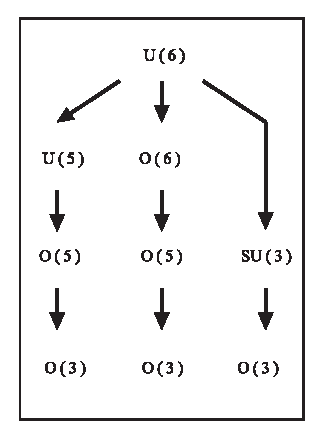
\includegraphics[scale=.65]{assets/figure}
		\caption{Figure with default placement}
		\label{01:fig:1}
	\end{figure}
	
	\begin{figure}[t]
		\sidecaption[t]
		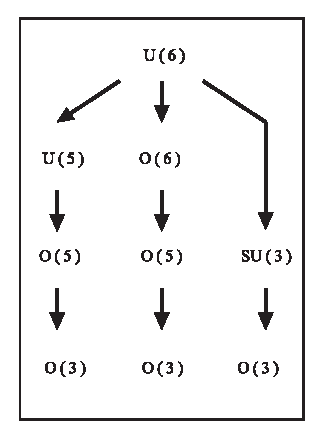
\includegraphics[scale=.65]{assets/figure}
		%
		% If no graphics program available, insert a blank space i.e. use
		%\picplace{5cm}{2cm} % Give the correct figure height and width in cm
		%
		\caption{Figure with column placement} % Note that this caption is printed in the list of figures, so keep it short.
		\label{01:fig:2}
	\end{figure}
	
	\paragraph{Paragraph Heading}\label{01:paragraph:1}
	
	For typesetting numbered lists we recommend to use the \verb|enumerate| environment -- it will automatically rendered in line with the layout.
	
	\begin{enumerate}
		\item{Livelihood and survival mobility are oftentimes coutcomes of uneven socioeconomic development.}
		\begin{enumerate}
			\item{Livelihood and survival mobility are oftentimes coutcomes of uneven socioeconomic development.}
			\item{Livelihood and survival mobility are oftentimes coutcomes of uneven socioeconomic development.}
		\end{enumerate}
		\item{Livelihood and survival mobility are oftentimes coutcomes of uneven socioeconomic development.}
	\end{enumerate}
	
	
	\subparagraph{Subparagraph Heading}\label{01:subparagraph:1:1}
	
	For unnumbered list we recommend to use the \verb|itemize| environment -- it will automatically be rendered in line with the layout.
	
	\begin{itemize}
		\item{Livelihood and survival mobility are oftentimes coutcomes of uneven socioeconomic development, cf. Table~\ref{01:tab:1}.}
		\begin{itemize}
			\item{Livelihood and survival mobility are oftentimes coutcomes of uneven socioeconomic development.}
			\item{Livelihood and survival mobility are oftentimes coutcomes of uneven socioeconomic development.}
		\end{itemize}
		\item{Livelihood and survival mobility are oftentimes coutcomes of uneven socioeconomic development.}
	\end{itemize}
	
	\runinhead{Run-in Heading Boldface Version} Use the \LaTeX\ automatism for all your cross-references and citations as has already been described in Sect.~\ref{01:subsection:2:1}.
	
	\subruninhead{Run-in Heading Boldface and Italic Version} Use the \LaTeX\ automatism for all your cross-references and citations as has already been described in Sect.~\ref{01:subsection:2:1}.
	
	\subsubruninhead{Run-in Heading Displayed Version} Use the \LaTeX\ automatism for all your cross-references and citations as has already been described in Sect.~\ref{01:subsection:2:1}.
	
	Use the \verb|\index{}| command to code your index words.
	
	For tables use \textbf{tabular} or \textbf{tabularx}.
	
	\begin{table}[!t]
		\caption{Please write your table caption here}
		\label{01:tab:1} % Give a unique label
		%
		% Follow this input for your own table layout
		%
		\begin{tabular}{p{2cm}p{2.4cm}p{2cm}p{4.9cm}}
			\hline\noalign{\smallskip}
			Classes & Subclass & Length & Action Mechanism  \\
			\noalign{\smallskip}\svhline\noalign{\smallskip}
			Translation & mRNA$^a$  & 22 (19--25) & Translation repression, mRNA cleavage\\
			Translation & mRNA cleavage & 21 & mRNA cleavage\\
			Translation & mRNA  & 21--22 & mRNA cleavage\\
			Translation & mRNA  & 24--26 & Histone and DNA Modification\\
			\noalign{\smallskip}\hline\noalign{\smallskip}
		\end{tabular}
		$^a$ Table foot note (with superscript)
	\end{table}
	%
	\section{Section Heading}\label{01:section:3}
	
	% Remember: Always give a unique label
	% and use \ref{<myprefix>:<label>} for cross-references
	% and \cite{<label>} for bibliographic references
	
	If you want to list definitions or the like we recommend to use the enhanced \verb|description| environment -- it will automatically rendered in line with the layout.
	
	\begin{description}[Type 1]
		\item[Type 1]{That addresses central themes pertainng to migration, health, and disease. In Sect.~\ref{01:section:1}, Wilson discusses the role of human migration in infectious disease distributions and patterns.}
		\item[Type 2]{That addresses central themes pertainng to migration, health, and disease. In Sect.~\ref{01:subsection:2:2}, Wilson discusses the role of human migration in infectious disease distributions and patterns.}
	\end{description}
	
	\subsection{Subsection Heading}\label{01:subsection:3:1}
	
	\lipsum
	
	\begin{svgraybox}
		If you want to emphasize complete paragraphs of texts we recommend to use the newly defined class option \verb|graybox| and the newly defined environment \verb|svgraybox|. This will produce a 15 percent screened box 'behind' your text.
		
		If you want to emphasize complete paragraphs of texts we recommend to use the newly defined class option and environment \verb|svgraybox|. This will produce a 15 percent screened box 'behind' your text.
	\end{svgraybox}
	
	
	\subsubsection{Subsubsection Heading}\label{01:subsubsection:3:1:1}
	
	\begin{theorem}
		Theorem text goes here.
	\end{theorem}
	
	
	\begin{problem}
		You can place a problem here.
	\end{problem}
	
	\begin{problem}{\nocaption}
		Another problem here.
	\end{problem}
	
	\begin{solution}
		And its solution here.
	\end{solution}
	
	\begin{definition}
		Definition text goes here.
	\end{definition}
	
	\begin{proof}
		Proof text goes here. \qed
	\end{proof}
	
	%% all available environments: claim, proof, case, conjecture, corollary, definition, example, exercise, lemma, note, problem, property, proposition, question, remark, solution, and theorem.
	
	\paragraph{Paragraph Heading} %
	Instead of simply listing headings of different levels we recommend to let every heading be followed by at least a short passage of text.  Further on please use the \LaTeX\ automatism for all your cross-references and citations as has already been described in Sect.~\ref{01:section:2}.
	
	Note that the first line of text that follows a heading is not indented, whereas the first lines of all subsequent paragraphs are.
	%
	% For built-in environments use
	%
	\begin{theorem}
		Theorem text goes here.
	\end{theorem}
	%
	\begin{definition}
		Definition text goes here.
	\end{definition}
	%
	\begin{proof}
		%\smartqed
		Proof text goes here.
		%\qed
	\end{proof}
	%
	\begin{trailer}{Trailer Head}
		If you want to emphasize complete paragraphs of texts in an \verb|Trailer Head| we recommend to
		use  \begin{verbatim}\begin{trailer}{Trailer Head}
		...
		\end{trailer}\end{verbatim}
	\end{trailer}
	%
	\begin{question}{Questions}
		If you want to emphasize complete paragraphs of texts in an \verb|Questions| we recommend to
		use  \begin{verbatim}\begin{question}{Questions}
		...
		\end{question}\end{verbatim}
	\end{question}
	\eject%
	\begin{important}{Important}
		If you want to emphasize complete paragraphs of texts in an \verb|Important| we recommend to
		use  \begin{verbatim}\begin{important}{Important}
		...
		\end{important}\end{verbatim}
	\end{important}
	%
	\begin{warning}{Attention}
		If you want to emphasize complete paragraphs of texts in an \verb|Attention| we recommend to
		use  \begin{verbatim}\begin{warning}{Attention}
		...
		\end{warning}\end{verbatim}
	\end{warning}
	
	If you want to emphasize complete paragraphs of texts in an \verb|Program Code| we recommend to
	use \textbf{programcode} or, more sophisticated, the listings package.
	
	\begin{programcode}{Program Code}
		
		\verb|\begin{programcode}{Program Code}|
		
		\verb|\begin{verbatim}...\end{verbatim}|
		
		\verb|\end{programcode}|
		
		or the listings package:
		
		\verb|\begin{lstlisting}[options]|
		\verb|...|
		\verb|\end{lstlisting}|
		
	\end{programcode}
	
	\begin{lstlisting}[language=Java,frame=single,caption={Sample Java Code},captionpos=b,label={01:listing:1}]
	println("this is listing code");
	\end{lstlisting}
	
	%
	\begin{tips}{Tips}
		If you want to emphasize complete paragraphs of texts in an \verb|Tips| we recommend to
		use  \begin{verbatim}\begin{tips}{Tips}
		...
		\end{tips}\end{verbatim}
	\end{tips}
	
	
	\begin{overview}{Overview}
		If you want to emphasize complete paragraphs of texts in an \verb|Overview| we recommend to
		use  \begin{verbatim}\begin{overview}{Overview}
		...
		\end{overview}\end{verbatim}
	\end{overview}
	\begin{backgroundinformation}{Background Information}
		If you want to emphasize complete paragraphs of texts in an \verb|Background|
		\verb|Information| we recommend to
		use
		
		\verb|\begin{backgroundinformation}{Background Information}|
		
		\verb|...|
		
		\verb|\end{backgroundinformation}|
	\end{backgroundinformation}
	\begin{legaltext}{Legal Text}
		If you want to emphasize complete paragraphs of texts in an \verb|Legal Text| we recommend to
		use  \begin{verbatim}\begin{legaltext}{Legal Text}
		...
		\end{legaltext}\end{verbatim}
	\end{legaltext}
	%
	\begin{acknowledgement}
		If you want to include acknowledgments of assistance and the like at the end of an individual chapter please use the \verb|acknowledgement| environment -- it will automatically be rendered in line with the layout.
	\end{acknowledgement}
	%
	
	\section*{Appendix}\label{01:appendix}
	\addcontentsline{toc}{section}{Appendix} % add to toc.
	
	You can place your appendix here, if needed. Note that you should not use the \verb|\appendix| comment, because it will continue numeric instead of alphabetical numbering from the main content. Alphabetical numbering is reserved for the global appendix. Use the starred versions of the section commands to suppress ongoing numbering. If you need multiple appendixes, name them "Appendix 1", "Appendix 2", and so on.
	
	\begin{equation}
	a \times b = c
	\end{equation}
	
	%%%%%%%%%%%%%%%%%%%%%%%%%%%%%%%%%%%%%%%%%%%%%%%%%%%%%%%%%%%%%%%%%%%%%%%%%%%%%%%%%%%%%%%%%%%%%%%%%%%%%%%%
	%% For your bibliography, you should use a bibtex .bib file and include it here.
	%% Note that the final reference lists styling might differ because it'll be styled in unified book layout.
	
	\biblstarthook{
		text inserted here will be printed before the actual list of references, but only if there is at least one reference to display. Delete this section if you don't need it.
	}
	
	%\nocite{*}		%% uncomment if uncited references should be listed in the bibliography.
	

	%% uncomment and state path to your .bib to use a bibtex file as your bibliography.
	%% NOTE: relative paths don't work in \putbib => During development, you might delete the "\CHAPTERSROOT/chapter01/" part to refer to your bib file. When you're done, please make this path absolute again by adding the prefix again (adjusting your chapter number).
	\putbib[\CHAPTERSROOT/chapter01/bibliography]
	
\end{bibunit}
	
%% uncomment the \end{document} statement to make this file stand-alone compileable.
%\end{document}